% =========================================================================
% SECTION 2.2: MPPT THEORY
% =========================================================================
\section{MPPT Theory}

\subsection{Introduction to MPPT}
Photovoltaic (PV) arrays are fundamentally non-linear power sources. Unlike a standard DC power supply or a battery, which can maintain a relatively stable voltage regardless of the load, the current and voltage output of a solar panel depends entirely on atmospheric conditions (solar irradiance and ambient temperature) and the electrical characteristic of the connected load.

If a PV module is connected directly to a fixed load (like a battery or a basic inverter input), the system will rarely operate at its maximum efficiency. The operating point will simply be the intersection of the load line and the PV module's Current-Voltage ($I$-$V$) curve. Because weather conditions change continuously throughout the day, this intersection point shifts, often forcing the solar panel to operate well below its true power capacity.

Maximum Power Point Tracking (MPPT) is an electronic control strategy, typically implemented within a DC-DC converter, designed to solve this exact problem. The primary purposes of an MPPT system are:

\begin{itemize}
    \item \textbf{Maximum Efficiency:} It continuously forces the PV array to operate at its Maximum Power Point (MPP), which is the unique point on the Power-Voltage ($P$-$V$) curve where the product of voltage ($V_{mpp}$) and current ($I_{mpp}$) yields the highest possible power output ($P_{max}$).
    \item \textbf{Impedance Matching:} By dynamically adjusting the duty cycle ($D$) of the switching power converter, the MPPT controller changes the \textit{apparent impedance} of the load as seen by the solar panel, matching it to the optimal internal impedance of the PV module.
    \item \textbf{Environmental Adaptation:} It ensures that even when clouds pass by or the temperature spikes (which drastically drops the panel's voltage output), the system instantly tracks the new peak power position without manual intervention.
\end{itemize}

\begin{figure}[H]
    \centering
    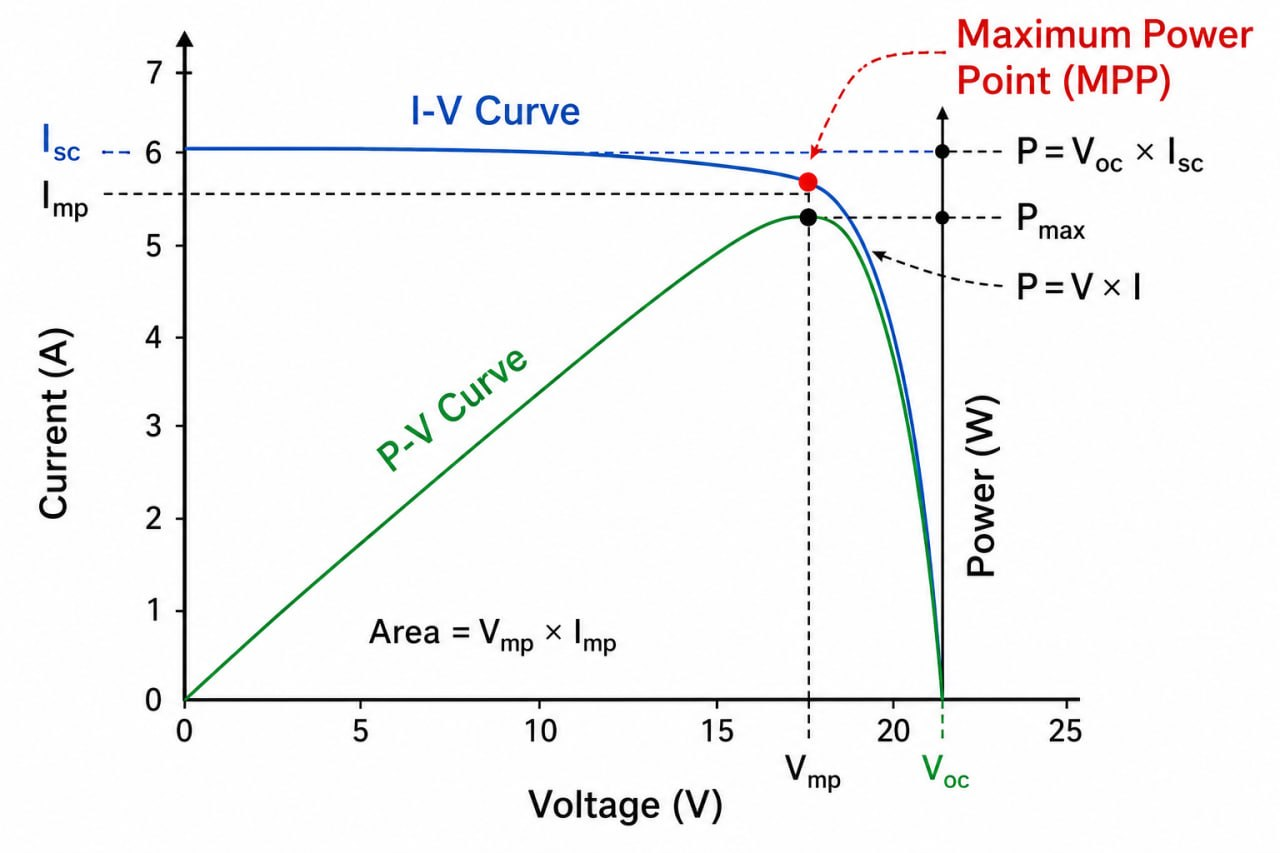
\includegraphics[width=0.7\textwidth]{Figures/Figure 2.16.jpg}
    \caption{P-V and I-V Characteristic Curves of a Photovoltaic Module.}
    \label{fig:pv_iv_curves}
\end{figure}

\subsection{Numerical Example of Power Tracking}
To understand how an MPPT algorithm tracks the peak power dynamically, we can analyze the behavior of a solar panel as its operating point shifts along the Power-Voltage ($P$-$V$) curve. Let us assume a starting condition and observe how changes in voltage ($V$) and current ($I$) affect the total output power ($P = V \times I$):

\begin{itemize}
    \item \textbf{Point 1 (Initial State):} The system operates at a voltage $V_1 = 20\text{ V}$ and a current $I_1 = 10\text{ A}$.
    \begin{equation}
        P_1 = 20\text{ V} \times 10\text{ A} = 200\text{ W}
    \end{equation}
    \item \textbf{Point 2 (Moving Up the Curve):} The algorithm changes the duty cycle, causing the voltage to slightly decrease to $V_2 = 19\text{ V}$, which allows the current to rise to $I_2 = 11\text{ A}$.
    \begin{equation}
        P_2 = 19\text{ V} \times 11\text{ A} = 209\text{ W}
    \end{equation}
    \textit{Observation:} Because $P_2 > P_1$ ($209\text{ W} > 200\text{ W}$), the power has \textit{increased}. This informs the controller that it is moving in the right direction toward the peak.
    \item \textbf{Point 3 (Past the Peak / Decreasing):} The algorithm attempts to change the operating point further in the same direction. The voltage drops to $V_3 = 17\text{ V}$, and the current rises to $I_3 = 12\text{ A}$.
    \begin{equation}
        P_3 = 17\text{ V} \times 12\text{ A} = 204\text{ W}
    \end{equation}
    \textit{Observation:} Because $P_3 < P_2$ ($204\text{ W} < 209\text{ W}$), the power has now \textit{decreased}. The controller realizes it has overshot the peak and must turn back toward Point 2.
\end{itemize}

\subsection{The Core Mathematical Condition}
This trial-and-error process is mathematically defined by analyzing the slope of the $P$-$V$ curve, which is the derivative of power with respect to voltage ($\frac{dP}{dV}$). As seen in the numerical example, the slope tells the controller exactly where it is relative to the Maximum Power Point (MPP):

\begin{itemize}
    \item \textbf{To the Left of the MPP ($\frac{dP}{dV} > 0$):} As voltage increases, power increases (this happened between Point 1 and Point 2). The controller needs to increase the voltage to reach the peak.
    \item \textbf{To the Right of the MPP ($\frac{dP}{dV} < 0$):} As voltage increases, power decreases (this happened when moving to Point 3). The controller needs to decrease the voltage to go back to the peak.
    \item \textbf{At the Maximum Power Point ($\frac{dP}{dV} = 0$):} The slope becomes perfectly flat. This is the ideal operating point ($P_{max} = 209\text{ W}$ in our example), where the system achieves maximum efficiency.
\end{itemize}

\begin{equation}
    \frac{dP}{dV} = 0
\end{equation}

\begin{figure}[H]
    \centering
    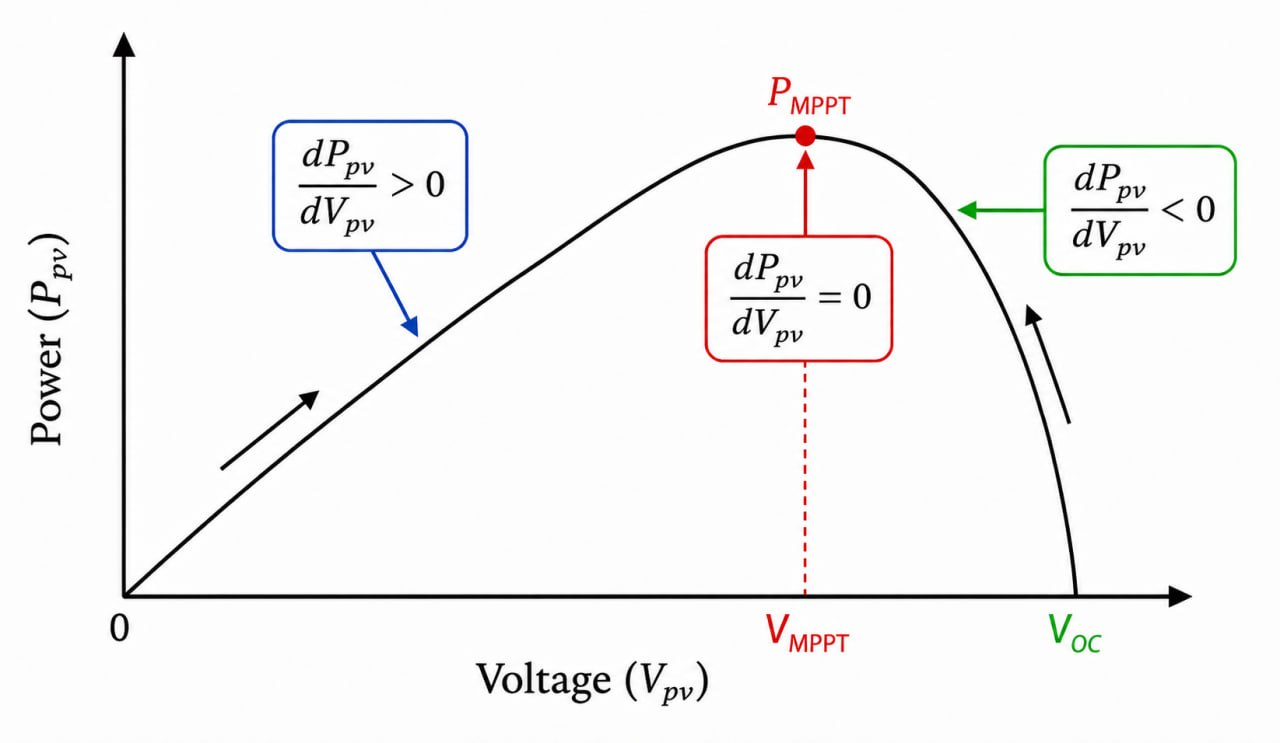
\includegraphics[width=0.65\textwidth]{Figures/Figure 2.17.jpg}
    \caption{MPPT Algorithm Operation Modes on the P-V Curve.}
    \label{fig:mppt_operation}
\end{figure}

\subsection{Classification of MPPT Algorithms}
To successfully satisfy the condition $\frac{dP}{dV} = 0$, various control strategies have been developed. These algorithms differ in complexity, tracking speed, sensor requirements, and their ability to handle uniform versus non-uniform solar irradiance.

\subsubsection{Perturb and Observe (P\&O)}
The Perturb and Observe (P\&O) algorithm, also known as the ``hill-climbing'' method, is the most widely used conventional MPPT technique due to its simplicity and low computational cost.

\paragraph{Operating Principle:}
The controller introduces a small perturbation (a deliberate step change) in the operating voltage of the PV array by modifying the converter's duty cycle, then measures the resulting power output. If the power increases ($\Delta P > 0$), the controller knows the perturbation moved the operating point closer to the peak and will continue to perturb the voltage in the \textit{same direction}. If the power decreases ($\Delta P < 0$), it means the operating point has overshot the peak, and the controller must \textit{reverse the direction} of the next perturbation.

\paragraph{Drawbacks:}
\begin{enumerate}
    \item \textbf{Steady-State Oscillation:} Once the algorithm reaches the true MPP, it cannot sit perfectly still. It continually perturbs the voltage back and forth across the peak, causing a small but constant power loss.
    \item \textbf{Tracking Failure under Rapid Weather Fluctuations:} If solar irradiance changes abruptly, the algorithm can get confused, tracking in the wrong direction and moving far away from the actual MPP.
\end{enumerate}

\begin{figure}[H]
    \centering
    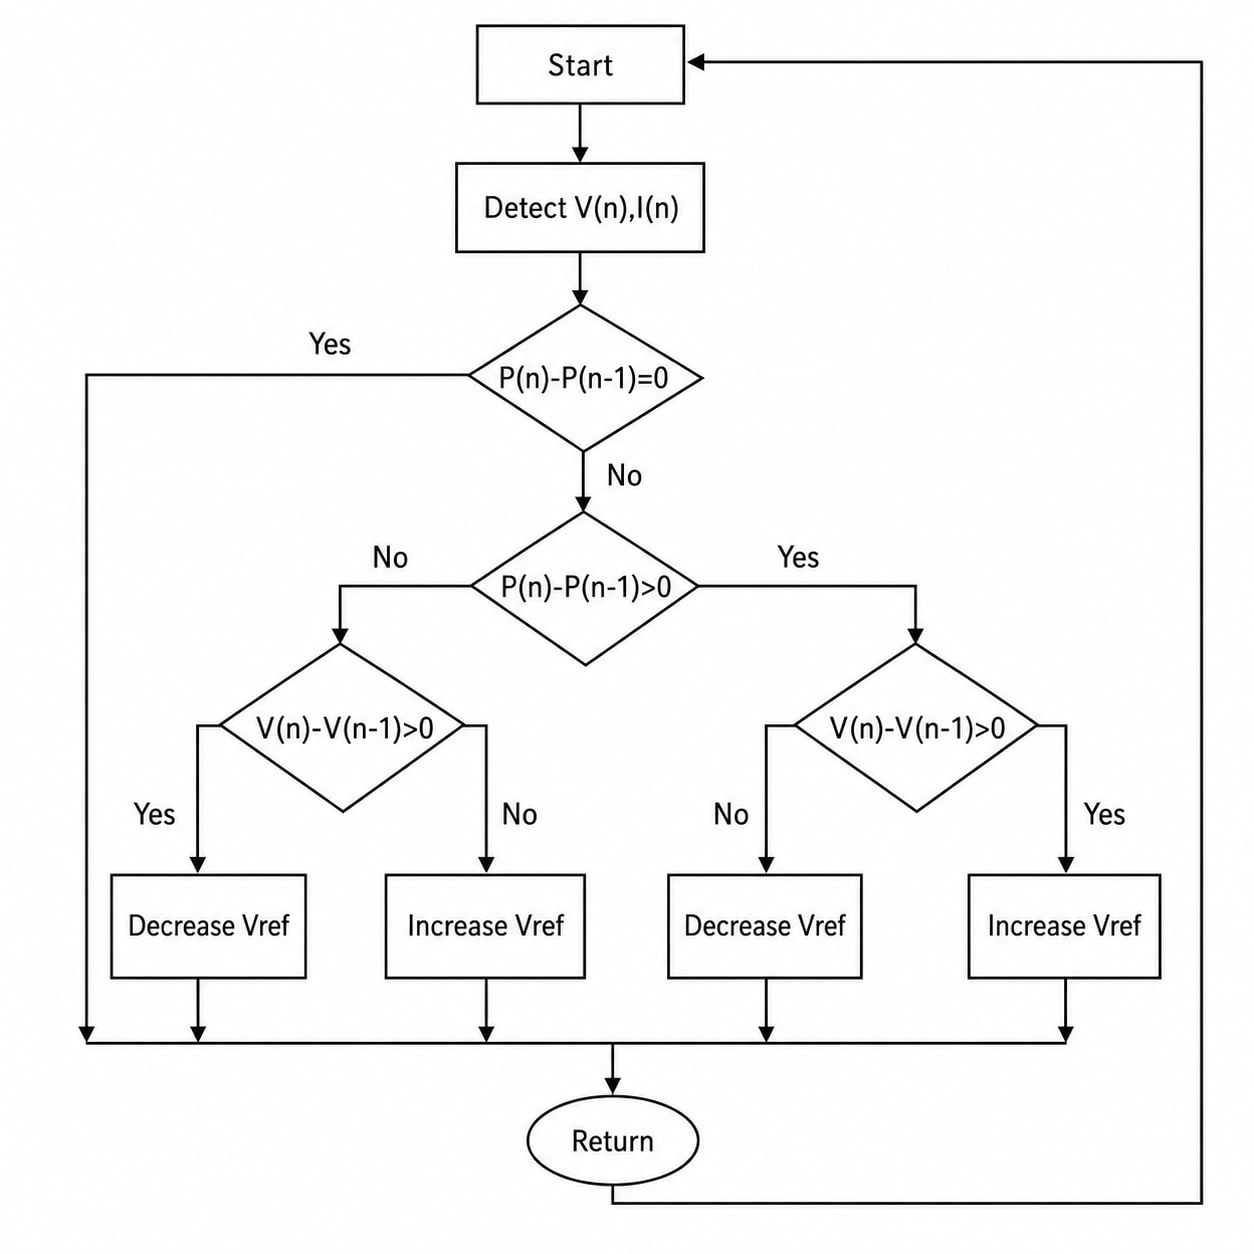
\includegraphics[width=0.6\textwidth]{Figures/Figure 2.18.jpg}
    \caption{Perturb and Observe (P\&O) Algorithm Flowchart.}
    \label{fig:po_flowchart}
\end{figure}

\subsubsection{Incremental Conductance (IncCond)}
The Incremental Conductance algorithm was designed to overcome the steady-state oscillation problem of P\&O. It uses the relationship between the instantaneous conductance ($\frac{I}{V}$) and the incremental conductance ($\frac{dI}{dV}$). As derived from the derivative of power ($P = VI$):

\begin{equation}
    \frac{dP}{dV} = I + V\frac{dI}{dV}
\end{equation}

By setting $\frac{dP}{dV} = 0$ at the maximum power point, the governing conditions are established as:
\begin{align}
    \frac{dI}{dV} &= -\frac{I}{V} \quad \text{(At the MPP)} \\
    \frac{dI}{dV} &> -\frac{I}{V} \quad \text{(Left of the MPP)} \\
    \frac{dI}{dV} &< -\frac{I}{V} \quad \text{(Right of the MPP)}
\end{align}

\paragraph{Operating Principle:}
The controller tracks the peak by comparing these two values. The major advantage of Incremental Conductance is that \textit{at the MPP, the perturbation stops completely}. The system maintains that exact operating point until a change in current ($\Delta I \neq 0$) is detected due to changing weather conditions.

\subsubsection{Global Scanning / Particle Swarm Optimization (PSO)}
Conventional methods like P\&O and IncCond assume the $P$-$V$ curve has only one single peak. However, if the EV charging station encounters \textit{Partial Shading} (e.g., a tree, building, or cloud casts a shadow over only part of the array), the $P$-$V$ curve warps. It creates multiple local peaks (Local MPPs) but only one true global peak (Global MPP).

\paragraph{The Problem with P\&O/IncCond:}
If a standard P\&O controller lands on a small local peak, it sees that $\frac{dP}{dV} = 0$. It gets stuck there indefinitely, completely missing the much larger global peak further down the curve.

\paragraph{The Global Scanning Solution:}
Soft-computing techniques like Particle Swarm Optimization (PSO) or global voltage sweeping algorithms send out ``scouts'' (virtual particles or rapid duty-cycle sweeps) across the entire voltage range from $0\text{ V}$ to $V_{oc}$. It scans the entire curve, identifies the absolute highest peak, and forces the converter to operate directly at the Global MPP.

\begin{figure}[H]
    \centering
    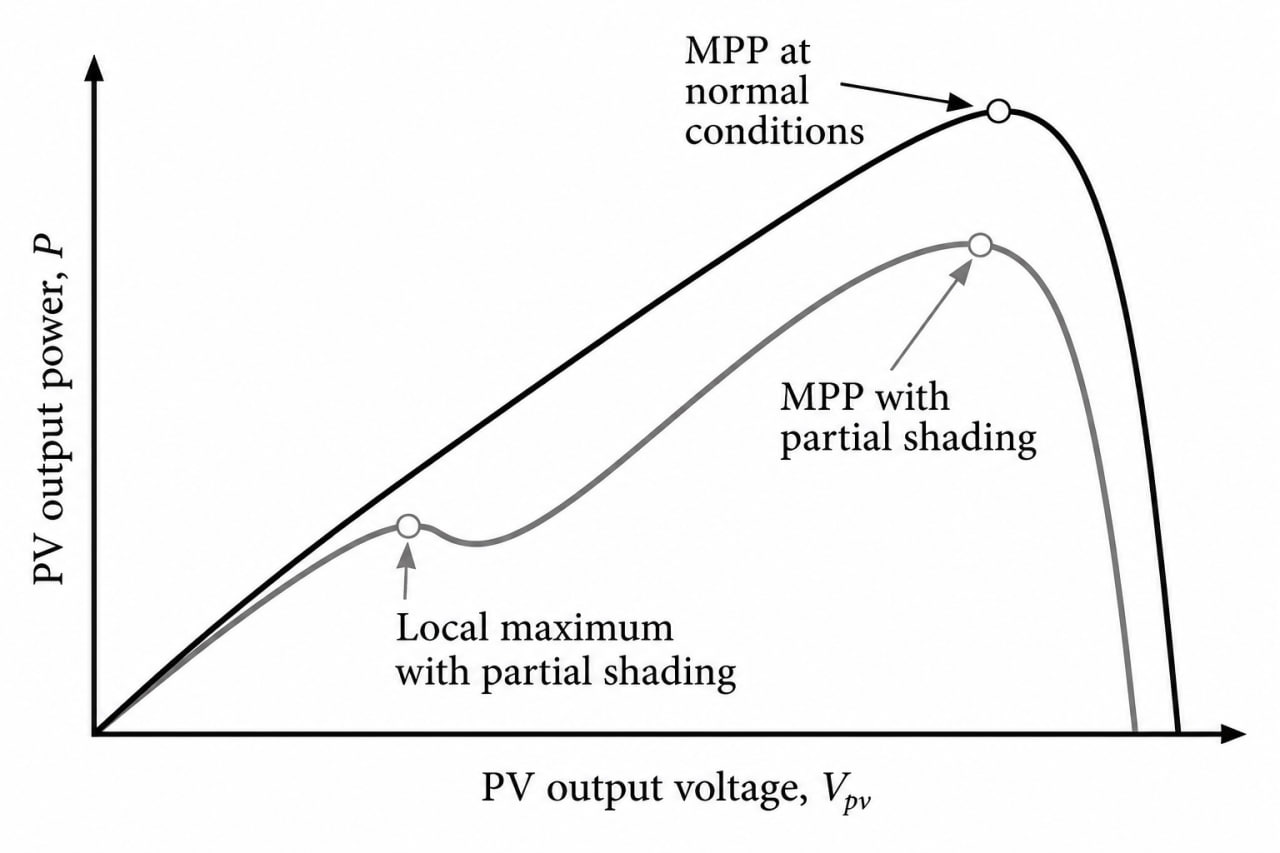
\includegraphics[width=0.7\textwidth]{Figures/Figure 2.19.jpg}
    \caption{Photovoltaic P-V Curve Characteristic Under Partial Shading Conditions.}
    \label{fig:global_vs_local}
\end{figure}

\newpage

\subsection{Advanced Concepts in Engineering Performance}

\subsubsection{Speed vs. Accuracy: Dynamic Efficiency}
In practical photovoltaic applications, atmospheric conditions are rarely static. On overcast days or during rapid cloud movement, solar irradiance can fluctuate drastically within a matter of seconds. This introduces the concept of \textit{Dynamic Efficiency}, which measures the MPPT controller's capability to track rapid variations in solar irradiance, converge on the newly established MPP in the shortest time possible, and maintain system stability without inducing severe oscillations. Balancing fast tracking speed with steady-state tracking accuracy is the absolute core of good engineering design.

\subsubsection{The Cost of Global Scanning (Global Sweep)}
While global scanning techniques are essential to locate the absolute highest peak under partial shading, executing them comes at a distinct energy cost. To search for the Global MPP, the controller must sweep the entire operating range of the PV array, moving from the open-circuit voltage ($V_{oc}$) down to the short-circuit current ($I_{sc}$).

\paragraph{The Engineering Problem:}
During this scanning period (which typically lasts between 1 to 5 seconds depending on the processor speed), the system is forced away from its optimal operating point. Consequently, the output power drops sharply during the sweep.

\paragraph{The Engineering Solution:}
To avoid continuous power layout degradation, the global sweep is not run constantly. Instead, it is programmed at a specific \textit{Periodic Sweep Interval} (e.g., every 10 to 30 minutes). This interval is engineered based on the geographical site conditions and shading patterns, representing a fine engineering trade-off between tracking accuracy and scanning losses.

\subsubsection{Power Conservation and Converter Efficiency}
A common misconception is that an MPPT controller inherently ``creates'' extra electrical energy. In reality, the MPPT operates strictly under the law of conservation of energy using a DC-DC power converter. Assuming an ideal power converter where internal switching losses are neglected, the input power extracted from the solar panels must equal the output power delivered to the load:

\begin{align}
    P_{in} &= P_{out} \\
    V_{in} \times I_{in} &= V_{out} \times I_{out}
\end{align}

\newpage

Based on this fundamental relationship, if the power converter acts to reduce the voltage from $40\text{ V}$ at the input to $20\text{ V}$ at the output, the output current must approximately double to conserve total power:
\begin{equation}
    \text{If } V_{out} = \frac{1}{2}V_{in} \implies I_{out} \approx 2 \times I_{in}
\end{equation}
Therefore, the MPPT does not generate additional power; rather, it dynamically reshapes the voltage-to-current relationship to perfectly match the load demands, optimizing overall system performance.

\subsection{Practical Efficiency and System Limitations}

\subsubsection{Real-World MPPT Efficiency and Loss Mechanisms}
In practical applications, even the most advanced MPPT controllers cannot achieve 100\% efficiency. The power losses within an MPPT system are primarily categorized into:
\begin{itemize}
    \item \textbf{Switching Losses:} Occurring during the high-frequency turn-on and turn-off transitions of power semiconductor switches such as MOSFETs and IGBTs.
    \item \textbf{Core Losses (Eddy Currents):} Occurring within the magnetic cores of inductors and transformers due to alternating magnetic fields.
    \item \textbf{Conduction Losses:} Resulting from the internal DC resistance ($R_{DS(on)}$) of switches, as well as the equivalent series resistance (ESR) of inductors and wiring.
    \item \textbf{Capacitive and Component Mating Losses:} Minor energy dissipation within filtering capacitors and auxiliary electronic components.
\end{itemize}
In modern industrial and commercial systems, the actual efficiency of an MPPT controller ranges between $95\%$ and $99\%$, depending on the power rating, design topology, and real-time operating conditions.

\subsubsection{Practical Constraints and Inverter Clipping}
An MPPT controller does not operate with absolute freedom; it is strictly bounded by the physical and electrical limitations of the power converter:
\begin{itemize}
    \item \textbf{MPPT Voltage Range:} Every tracking device has a specified voltage window (e.g., $150\text{ V}$ to $450\text{ V}$). If environmental factors or temperature fluctuations cause the PV string voltage to drop below the minimum threshold, the controller will completely fail to track the maximum power point.
    \item \textbf{Current Clipping:} Modern ultra-high-power PV modules generate significant current (often $18\text{ A}$ or higher). If the input current exceeds the maximum allowable threshold of the inverter or tracker, the MPPT controller intentionally shifts the operating point toward a higher voltage. This deliberately reduces the current to protect the hardware, resulting in the sacrifice or ``clipping'' of available potential power.
\end{itemize}

\subsection{Control Architecture and Modern Technology Impact}

\subsubsection{The Role of the Closed-Loop Control Architecture}
Inside the digital signal processor (DSP) or microcontroller, the tracking process is managed via a distinct, closed-loop control system. It is functionally divided into two layers:
\begin{itemize}
    \item \textbf{The MPPT Algorithm:} Acts as the high-level decision-maker. It analyzes the $P$-$V$ curve and decides \textit{where} the optimal operating point reference ($V_{ref}$ or $I_{ref}$) should move.
    \item \textbf{The Inner Control Loop:} Acts as the executor. Typically utilizing a Proportional-Integral (PI) or Proportional-Integral-Derivative (PID) digital control technique, it dynamically adjusts the converter's duty cycle ($D$) to drive the system to that reference point smoothly and stably.
\end{itemize}

\subsubsection{Impact of Advanced Photovoltaic Module Technologies}
Modern innovations in solar panel manufacturing directly affect MPPT behavior:
\begin{itemize}
    \item \textbf{Half-Cut Cell Modules:} These modules are split into two parallel, independent sections. When partial shading occurs, the affected half operates independently, drastically reducing the formation of multiple local peaks on the $P$-$V$ curve. This simplifies the tracking process and allows standard MPPT algorithms to operate with higher efficiency.
    \item \textbf{Bifacial Modules:} These panels absorb direct sunlight from the front and reflected ambient light (Albedo) from the rear. Because rear irradiance fluctuates continuously based on surrounding ground conditions, it introduces micro-oscillations into the $P$-$V$ curve, imposing a heavier computational burden on the tracking speed and responsiveness of the MPPT controller.
\end{itemize}

\subsection{Conclusion of MPPT Theory}
In summary, Maximum Power Point Tracking (MPPT) serves as the critical electronic control layer required to overcome the fundamentally non-linear power characteristics of photovoltaic arrays. By dynamically adjusting the duty cycle of an integrated DC-DC power converter, an MPPT system executes continuous impedance matching. This control mechanism ensures that the solar array operates at its peak electrical output regardless of volatile ambient temperatures or shifting solar irradiance levels.
\\

Ultimately, a robustly engineered MPPT control architecture balances tracking speed with steady-state accuracy. This optimization layer is vital for maintaining the high dynamic efficiency and power conservation necessary for demanding infrastructure applications, such as solar-powered electric vehicle charging stations interacting with dynamic DC microgrids.